\part{Arrays and pointers}
\frame{\partpage}

\begin{frame}[fragile]{Arrays in C++}
    \begin{itemize}
        \item An \textbf{array} is a fixed-length sequence of elements of a particular type
        \item Not to be confused with a \textbf{vector}, which is a variable length sequence
    \end{itemize}
    \begin{lstlisting}
// Declare a 5-element array with initial values
int myArray[] = { 1, 3, 5, 7, 9 };

// Declare a 10-element array without specifying initial values
int myOtherArray[10];
    \end{lstlisting}
\end{frame}

\begin{frame}[fragile]{Arrays in memory}
    \begin{center}
        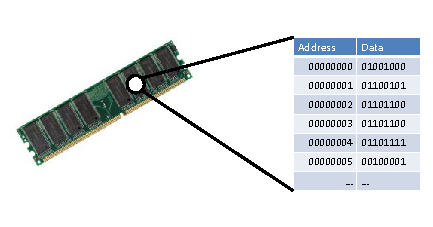
\includegraphics[width=0.6\textwidth]{memory.pdf}
    \end{center}
    \begin{itemize}
        \item An array is a contiguous block of memory
        \item E.g.\ an \lstinline{int} is 4 bytes (32 bits), so an array of 10 \lstinline{int}s is $10 \times 4 = 40$ bytes
        \item The size of the array is \textbf{fixed}: a 10 element array holds exactly 10 elements, forever
    \end{itemize}
\end{frame}

\begin{frame}[fragile]{Index out of range}
    This Python code will give a ``list index out of range'' exception
    \begin{lstlisting}[language=Python]
myList = [1, 3, 5, 7, 9]
print myList[5]
    \end{lstlisting}
    
    This C++ code will give a ``vector subscript out of range'' exception
    \begin{lstlisting}
std::vector<int> myVector = {1, 3, 5, 7, 9};
std::cout << myVector[5] << std::endl;
    \end{lstlisting}
    
    This C++ code will print some arbitrary number
    \begin{lstlisting}
int myArray[] = { 1, 3, 5, 7, 9 };
std::cout << myArray[5] << std::endl;
    \end{lstlisting}
\end{frame}

\begin{frame}[fragile]{Index out of range}
    \begin{itemize}
        \item C++ does not check array indices
        \item It is easy to accidentally read or write past the end of the array, and doing so will cause
            hard-to-fix bugs
        \item \lstinline{myArray} is a 5-element array of \lstinline{int}s, i.e.\ a block of $5 \times 4 = 20$ bytes
        \item If \lstinline{myArray} starts at memory address $1000$, then \lstinline{myArray[i]} is at address
            $1000 + 4 \times i$
        \item \lstinline{myArray[5]} is whatever happens to be at memory address $1000 + 4 \times 5 = 1020$ ---
            could be unallocated memory, could be another variable, could be part of another array,
            could even be part of the machine code being executed
    \end{itemize}
\end{frame}

\begin{frame}[fragile]{Array size must be a compile-time constant}
    \begin{lstlisting}
double a[10];            // OK

const int size = 10;
double b[size];          // OK
double c[2 * size + 7];  // OK

int varSize = 10;
double d[varSize];       // Error
    \end{lstlisting}
\end{frame}

\begin{frame}[fragile]{Dynamic allocation}
    \begin{itemize}
        \item If the size of the array is not known in advance, it can be allocated at runtime
            using the \lstinline{new} keyword
    \end{itemize}
    \begin{lstlisting}
int n = readNumberFromConsole();
int* myArray = new int[n];
    \end{lstlisting}
    \begin{itemize}
        \item Technically \lstinline{myArray} is no longer an array, it's a \textbf{pointer}
        \item \lstinline{int*} is the type ``pointer to an \lstinline{int}''
        \item Pointers can (mostly) be used as if they were arrays
    \end{itemize}
\end{frame}

\begin{frame}[fragile]{Stack and heap}
    \begin{itemize}
        \item Variables and static arrays are stored on the \textbf{stack}
        \begin{itemize}
            \item Stack items are automatically freed when they go out of scope
        \end{itemize}
        \item Anything created with \lstinline{new} is stored on the \textbf{heap}
        \begin{itemize}
            \item Heap items must be freed with \lstinline{delete} when they are finished with
            \item Forgetting to free them is a \textbf{memory leak}
        \end{itemize}
    \end{itemize}
\end{frame}

\begin{frame}[fragile]{Strings revisited}
    \begin{itemize}
        \item \lstinline{std::string} is the high-level string class
        \item The low-level way of storing strings is as an array of \lstinline{char}s
    \end{itemize}
    \begin{lstlisting}
char greeting[] = "Hello, world!";
    \end{lstlisting}
    \begin{itemize}
        \item Strings are \textbf{null terminated} --- they end with ASCII character 0
    \end{itemize}
\end{frame}

\begin{frame}[fragile]{String literals}
    \begin{lstlisting}
std::string greeting = "Hello, world!";
    \end{lstlisting}
    \begin{itemize}
        \item The thing on the right hand side is actually a \lstinline{char} array, not a \lstinline{std::string}
        \item The assignment operator knows how to convert from \lstinline{char[]} to \lstinline{std::string}
    \end{itemize}
\end{frame}

%\begin{frame}[fragile]{Pointers}
%    \begin{itemize}
%        \item C++ allows us to store and manipulate \textbf{pointers} a.k.a.\ memory addresses
%    \end{itemize}
%    \begin{lstlisting}
%int myVar = 7;
%int* myPointer = &myVar;
%*myPointer = 12;
%    \end{lstlisting}
%    \begin{itemize}
%        \item \lstinline{int*} is a type: pointer to int
%        \item \lstinline{&} is the \textbf{address-of} operator:
%            read \lstinline{&myVar} as ``a pointer to \lstinline{myVar}''
%        \item \lstinline{*} on line 3 is the \textbf{dereference} operator:
%            read \lstinline{*myPointer} as ``the value pointed to by \lstinline{myPointer}''
%    \end{itemize}
%\end{frame}

\begin{frame}[fragile]{2-dimensional arrays}
    Array of arrays approach:
    \begin{lstlisting}
const int width = 8, height = 8;
int grid[width][height];
grid[x][y] = 7;
    \end{lstlisting}
    Flat array approach:
    \begin{lstlisting}
const int width = 8, height = 8;
int grid[width * height];
grid[x + y * width] = 7;
    \end{lstlisting}
\end{frame}

